\documentclass{IEEEoj-data}
\usepackage{cite}
\usepackage{amsmath,amssymb,amsfonts}
\usepackage{graphicx,color}
\usepackage{textcomp}
\usepackage{hyperref}
\usepackage{balance}
\usepackage{listings}
\usepackage[T1]{fontenc}
\usepackage[normalem]{ulem}
\usepackage[draft]{changes}
\setaddedmarkup{\textcolor{blue}{\uline{#1}}}
\setdeletedmarkup{\textcolor{red}{\sout{#1}}}

\lstset{
  basicstyle=\ttfamily\footnotesize,
  breaklines=true,
  frame=single,
  framesep=3pt,
  xleftmargin=5pt,
  xrightmargin=5pt,
}

\AtBeginDocument{\definecolor{ojcolor}{cmyk}{0.93,0.59,0.15,0.02}}

\begin{document}

\title{\textcolor{black}{Descriptor:} \textcolor{ieeedata}{\textit{ AEGIS\deleted{\texttrademark{}} Threat Matrix for Agentic AI Systems (ATX-1)}}}

\author{KENNETH TANNENBAUM\authorrefmark{1} (MEMBER, IEEE)}
\affil{AEGIS Initiative, Lovettsville, Virginia, USA}
\corresp{CORRESPONDING AUTHOR: Kenneth Tannenbaum (e-mail: ktannenbaum@aegis-initiative.com).}
\authornote{This work was done independently of any grants or awards, produced under AEGIS Operations LLC. ORCID: 0009-0007-4215-1789.}
\markboth{DESCRIPTOR: AEGIS THREAT MATRIX FOR AGENTIC AI SYSTEMS (ATX-1)}{TANNENBAUM}

\begin{abstract}
ATX-1 (AEGIS Threat Matrix) is a structured adversarial knowledge base that catalogs failure modes of autonomous AI agents operating without governance constraints. Unlike existing threat frameworks---MITRE ATT\&CK for human adversaries and MITRE ATLAS for adversaries targeting AI systems---ATX-1 addresses a distinct threat class: AI agents that act outside their governance boundaries not through external compromise, but through their own structural capability without corresponding authority. ATX-1 is grounded in a fundamental distinction: capability---what an agent can do---is not authority---what an agent may do. The \replaced{five}{four} structural root causes identified in the dataset (missing authority verification, missing consequence modeling, missing behavioral boundaries, \replaced{missing state integrity protection, and missing environment model}{and missing state integrity protection}) trace all \replaced{29 techniques (and 29 sub-techniques)}{20 techniques} to architectural gaps that governance frameworks can address. The dataset defines \replaced{10 tactics (TA001--TA010)}{9 tactics (TA001--TA009)}, \replaced{29 techniques with 29 sub-techniques distributed non-sequentially across tactics (T1001--T10004 with sub-techniques T\#\#\#\#.\#\#\#)}{20 techniques distributed non-sequentially across tactics (T1001--T9001)}, and \replaced{29 mitigations}{20 mitigations}, each grounded in empirical observations from the {\it Agents of Chaos} study, which documented 11 failure modes across live agentic deployments. ATX-1 is published in STIX 2.1 format for compatibility with threat intelligence platforms, with supplementary structured JSON files providing technique metadata, regulatory cross-references to the NIST AI Risk Management Framework, EU AI Act, and OWASP Top 10 for LLM Applications, and a JSON Schema for validation. The dataset satisfies FAIR principles through three permanent repositories---IEEE DataPort, Zenodo, and a live machine-readable API---under the Apache 2.0 license.\\
\\
{\textcolor{ieeedata}{\abstractheadfont\bfseries{IEEE SOCIETY/COUNCIL}}} Computer Society (CS)\\
\\
{\textcolor{ieeedata}{\abstractheadfont\bfseries{DATA DOI/PID}}} \replaced{10.5281/zenodo.20171712 (ATX-1 v2.3)}{10.21227/f87b-1d57 (ATX-1 v1.0)}\\

{\textcolor{ieeedata}{\abstractheadfont\bfseries{DATA TYPE/LOCATION}}} Threat Taxonomy; Online (IEEE DataPort, Zenodo, aegis-governance.com)
\end{abstract}

\begin{IEEEkeywords}
Agentic AI, AI governance, autonomous agents, constitutional enforcement, EU AI Act, NIST AI RMF, OWASP LLM, STIX 2.1, threat taxonomy
\end{IEEEkeywords}

\maketitle

\section*{BACKGROUND}

Autonomous AI agents---systems that execute real-world actions against operational infrastructure including API calls, file system operations, database queries, and inter-service requests---have grown significantly in production deployments during the \replaced{eighteen}{twelve} months preceding this publication~\cite{ref1}. This growth has outpaced the development of governance infrastructure suited to the action layer, creating a systematic gap between what agents can do and what they are authorized to do.

Existing threat taxonomy frameworks do not address this gap. MITRE ATT\&CK~\cite{ref2} catalogs adversarial tactics and techniques used by human threat actors against computer systems. MITRE ATLAS~\cite{ref3} catalogs adversarial tactics used against AI and machine learning systems. Both frameworks model a clear attacker-target separation: an external adversary acts against a system. ATX-1 \replaced{addresses an adjacent and complementary failure surface: the failure modes that originate within the agent's own action path, regardless of whether the immediate trigger is an external input (e.g., indirect prompt injection) or an emergent property of the agent's reasoning under permissive conditions}{addresses the scenario where the AI agent itself is the threat source---not through compromise or malicious intent, but through capability without governance constraint}. \added{The distinction is not exclusionary: composite scenarios where adversarial inputs trigger ATX-1 failure modes are explicitly in scope, and a complete security posture for an agent deployment typically requires controls drawn from all three taxonomies. See the Definitions subsection below.}

\begin{figure*}[!t]
\centering
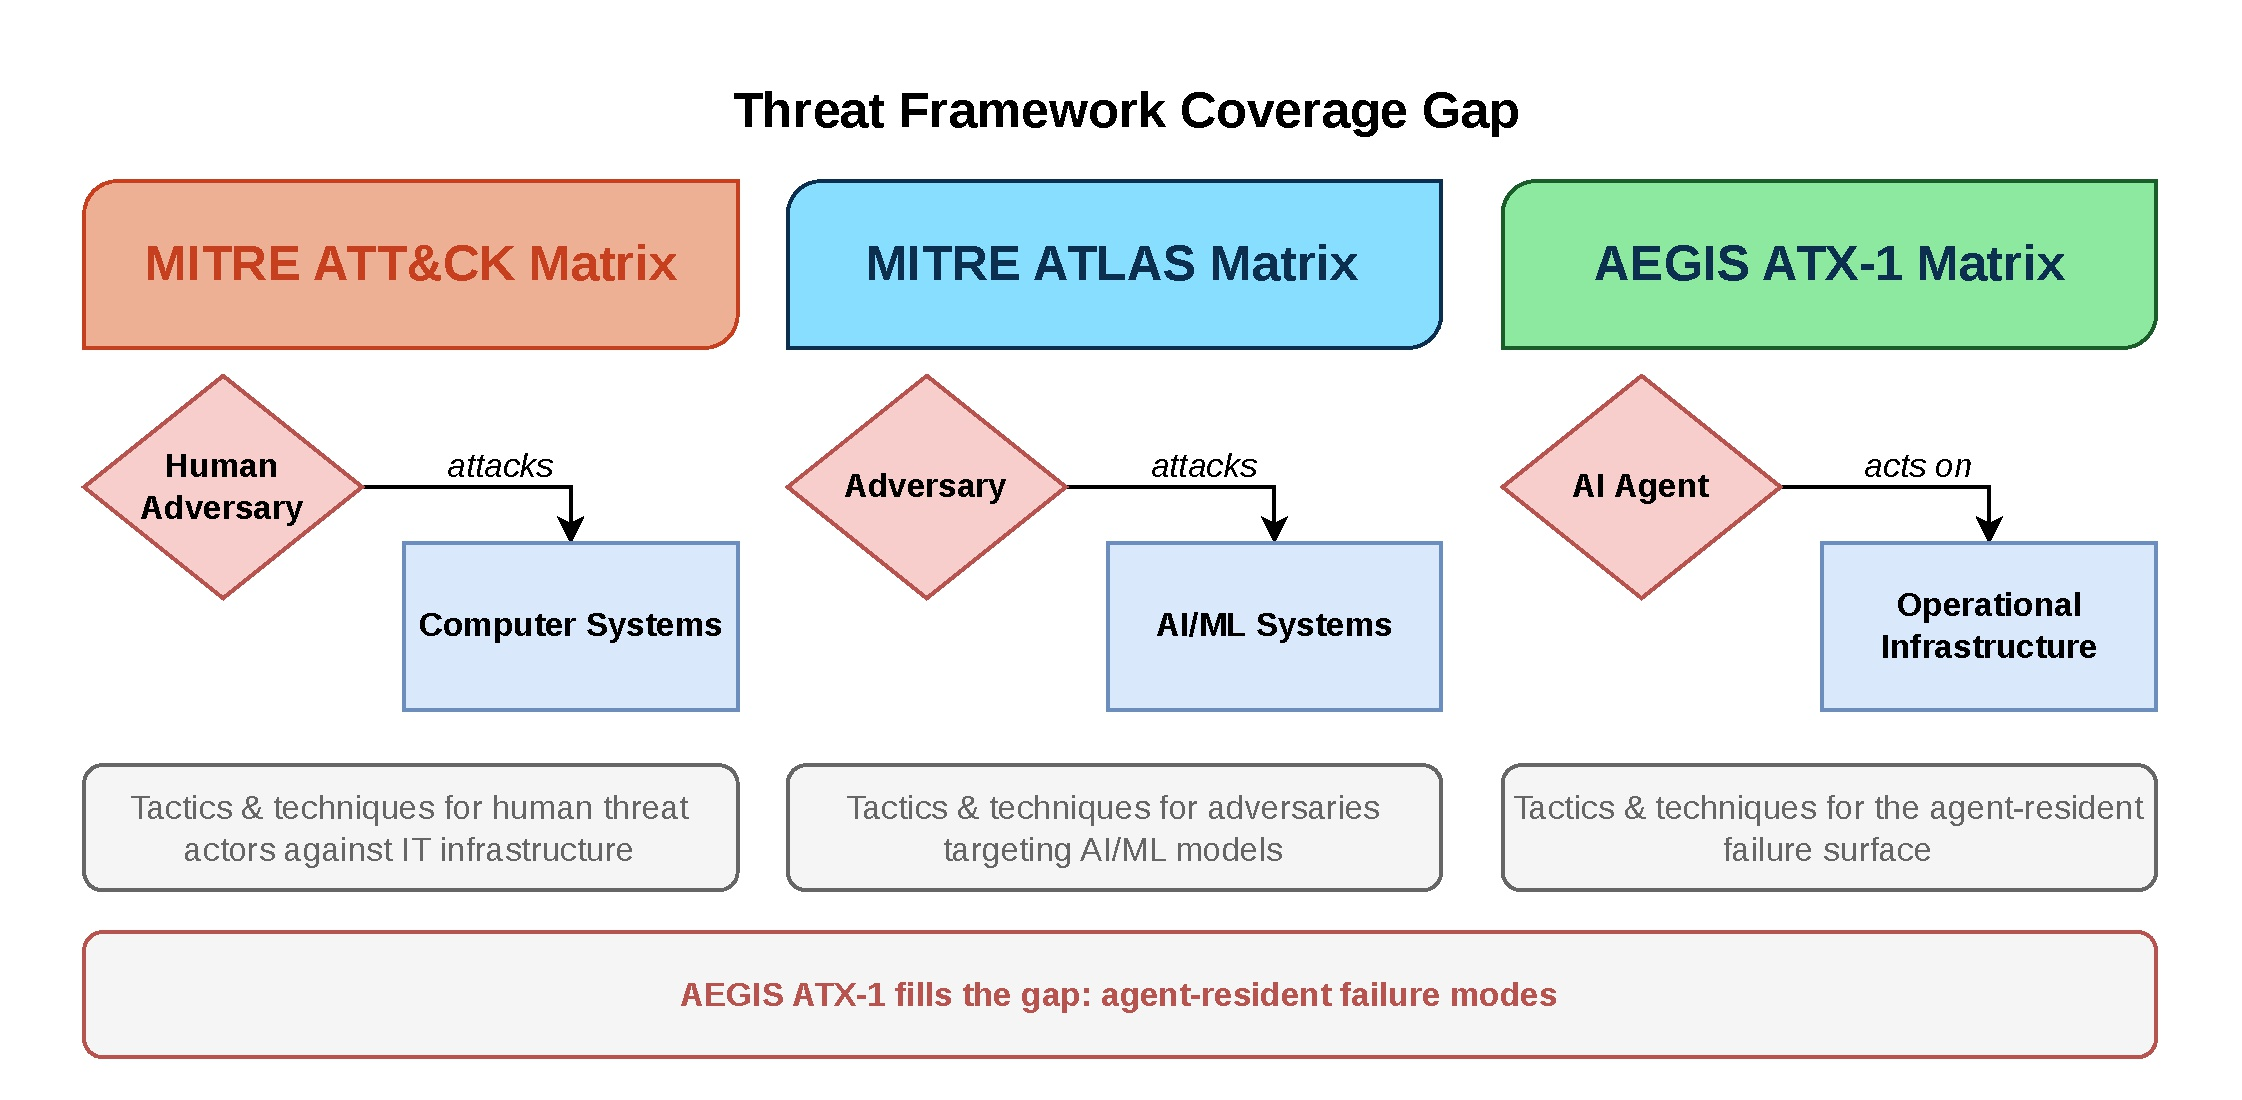
\includegraphics[width=\textwidth]{coverage-gap}
\caption{Threat framework coverage gap. MITRE ATT\&CK catalogs human adversaries attacking computer systems. MITRE ATLAS catalogs adversaries attacking AI/ML systems. ATX-1 addresses the uncovered scenario: AI agents \protect\replaced{whose own action path produces destructive outcomes (whether the immediate trigger is internal or external, e.g., indirect prompt injection that flows into the action layer)}{that act on operational infrastructure without governance constraint}. \protect\replaced{The three taxonomies are complementary, not mutually exclusive; a deployed agent system typically needs coverage from all three.}{The distinction between ``attacks'' and ``acts on'' reflects the structural difference---ATX-1 agents are not adversaries but ungoverned systems.}}
\label{fig:gap}
\end{figure*}

The distinction is structural. ATT\&CK and ATLAS model adversaries who attack systems. ATX-1 models the \replaced{agent-resident failure surface---the conditions under which an agent's own action path produces destructive outcomes regardless of whether the immediate trigger is internal (emergent under permissive conditions) or external (e.g., indirect prompt injection that flows through the agent's reasoning into the action layer)}{agents that are themselves the threat source---systems that delete data not because an attacker told them to, but because no architectural mechanism verified that the instruction source held the authority to request deletion}. The {\it Agents of Chaos} study (Shapira et al., 2026)~\cite{ref4} documented this failure pattern systematically, identifying 11 distinct failure modes across live agentic deployments involving 20 researchers over two weeks.

Multiple independent research groups have converged on the same finding. Arora et al.\ (2025) demonstrated that common multi-agent design patterns---including plan construction strategies, inter-agent context sharing, and fallback behaviors---carry significant vulnerabilities that emerge from architecture and interaction, not solely from adversarial prompts~\cite{ref11}. Ko et al.\ (2025) identified seven categories of security challenges in cross-domain multi-agent systems, establishing that ``a benign agent in isolation may leak secrets or violate policy'' when interacting with other agents across trust boundaries~\cite{ref12}. Reid et al.\ (2025) formalized six failure classes for governed multi-agent systems---including cascading failures, conformity bias, and mixed-motive dynamics---concluding that ``a collection of safe agents does not guarantee a safe collection''~\cite{ref13}. These studies independently corroborate the core premise of ATX-1: that agent-level safety does not ensure system-level safety, and that a distinct threat taxonomy is required for the agent-to-infrastructure action layer.

ATX-1 was developed as part of the AEGIS (Architectural Enforcement and Governance of Intelligent Systems) project~\cite{ref5}, an open governance architecture that applies reference monitor principles~\cite{ref14} to enforce deterministic constitutional policy at the agent action boundary. The taxonomy directly informs the AEGIS threat model (ATM-1) and maps each technique to specific constitutional articles and governance protocol mechanisms that mitigate it.

\replaced{While several recent efforts catalog agentic AI risks at a higher level---the OWASP Top 10 for Agentic Applications (December 2025)~\mbox{\cite{ref30}}, the Microsoft AI Red Team's {\it Taxonomy of Failure Modes in Agentic AI Systems} (April 2025)~\mbox{\cite{ref17}}, and MITRE ATLAS's agentic technique additions in v5.4.0 (February 2026)~\mbox{\cite{ref3}}---none provide a complete machine-readable dataset of agent-resident failure modes with technique-level detail, architectural mitigation mappings, and STIX 2.1 encoding. The OWASP Top 10s (LLM~\mbox{\cite{ref6}} and Agentic~\mbox{\cite{ref30}}) are categorical risk lists; the Microsoft Taxonomy is a narrative whitepaper; ATLAS focuses primarily on adversaries against AI systems rather than the agent-resident failure surface. ATX-1 occupies this gap.}{No comparable machine-readable dataset exists for agentic AI threat modeling. The OWASP Top 10 for LLM Applications~\mbox{\cite{ref6}} provides a high-level risk categorization but does not define individual techniques, map mitigations to architectural mechanisms, or provide STIX-compatible data for integration with threat intelligence platforms. ATX-1 fills this gap.}

\subsection*{\added{Definitions}}

\added{{\bf Agentic AI.} A system in which a large language model (or other AI mechanism) produces actions that execute against operational infrastructure---API calls, file-system operations, database queries, inter-service requests---without per-action human authorization. Humans set goals and constraints; the agent's reasoning loop selects individual actions and targets. AI-generated text or recommendations are not, by this definition, agentic; AI-invoked tool calls against systems, APIs, or files are.}

\added{{\bf Governance boundary.} The architectural point at which an agent's proposed actions are evaluated against policy and either allowed, denied, or escalated. The governance boundary sits between the agent's reasoning loop and the action surface; it is structurally distinct from training-time alignment (e.g., RLHF, Constitutional AI), which operates inside the model. Equivalent boundaries appear in classical security architectures: the reference monitor concept~\mbox{\cite{ref10}}, the policy-decision-point/policy-enforcement-point pattern, and runtime contract enforcement in service-oriented systems.}

\added{{\bf Threat source.} In ATT\&CK, the threat source is a human adversary external to the system. In ATLAS, the threat source is an adversary (external or internal) targeting an AI/ML system. In ATX-1, the threat source is the AI agent itself---not as an adversary but as a system whose structural capability exceeds its architectural authority. Composite scenarios are explicitly in scope: external adversarial inputs (e.g., indirect prompt injection) routinely trigger ATX-1 failure modes, and ATX-1 catalogs the agent-resident failure surface that such triggers exploit.}

\added{{\bf Capability and authority.} {\it Capability} is what an agent technically can do given its tool access, network reach, and execution permissions. {\it Authority} is the architectural representation of what the agent is permitted to do, conditioned on its identity, the action's principal, and the consequences. ATX-1 catalogs failure modes that arise from gaps in this distinction.}

\added{{\bf Scope (not exclusionary).} ATX-1 v2.3 is complementary, not exclusionary. A production agent deployment will routinely encounter composite risk scenarios that combine adversarial inputs with structural agent vulnerabilities; a complete security posture requires controls drawn from ATX-1 (agent-resident failure modes), ATT\&CK (human adversaries against the supporting infrastructure), and ATLAS (adversaries against the agent's model or pipeline). Practitioners should treat the three taxonomies as a layered defense, not as competing accounts.}

\begin{figure*}[!t]
\centering
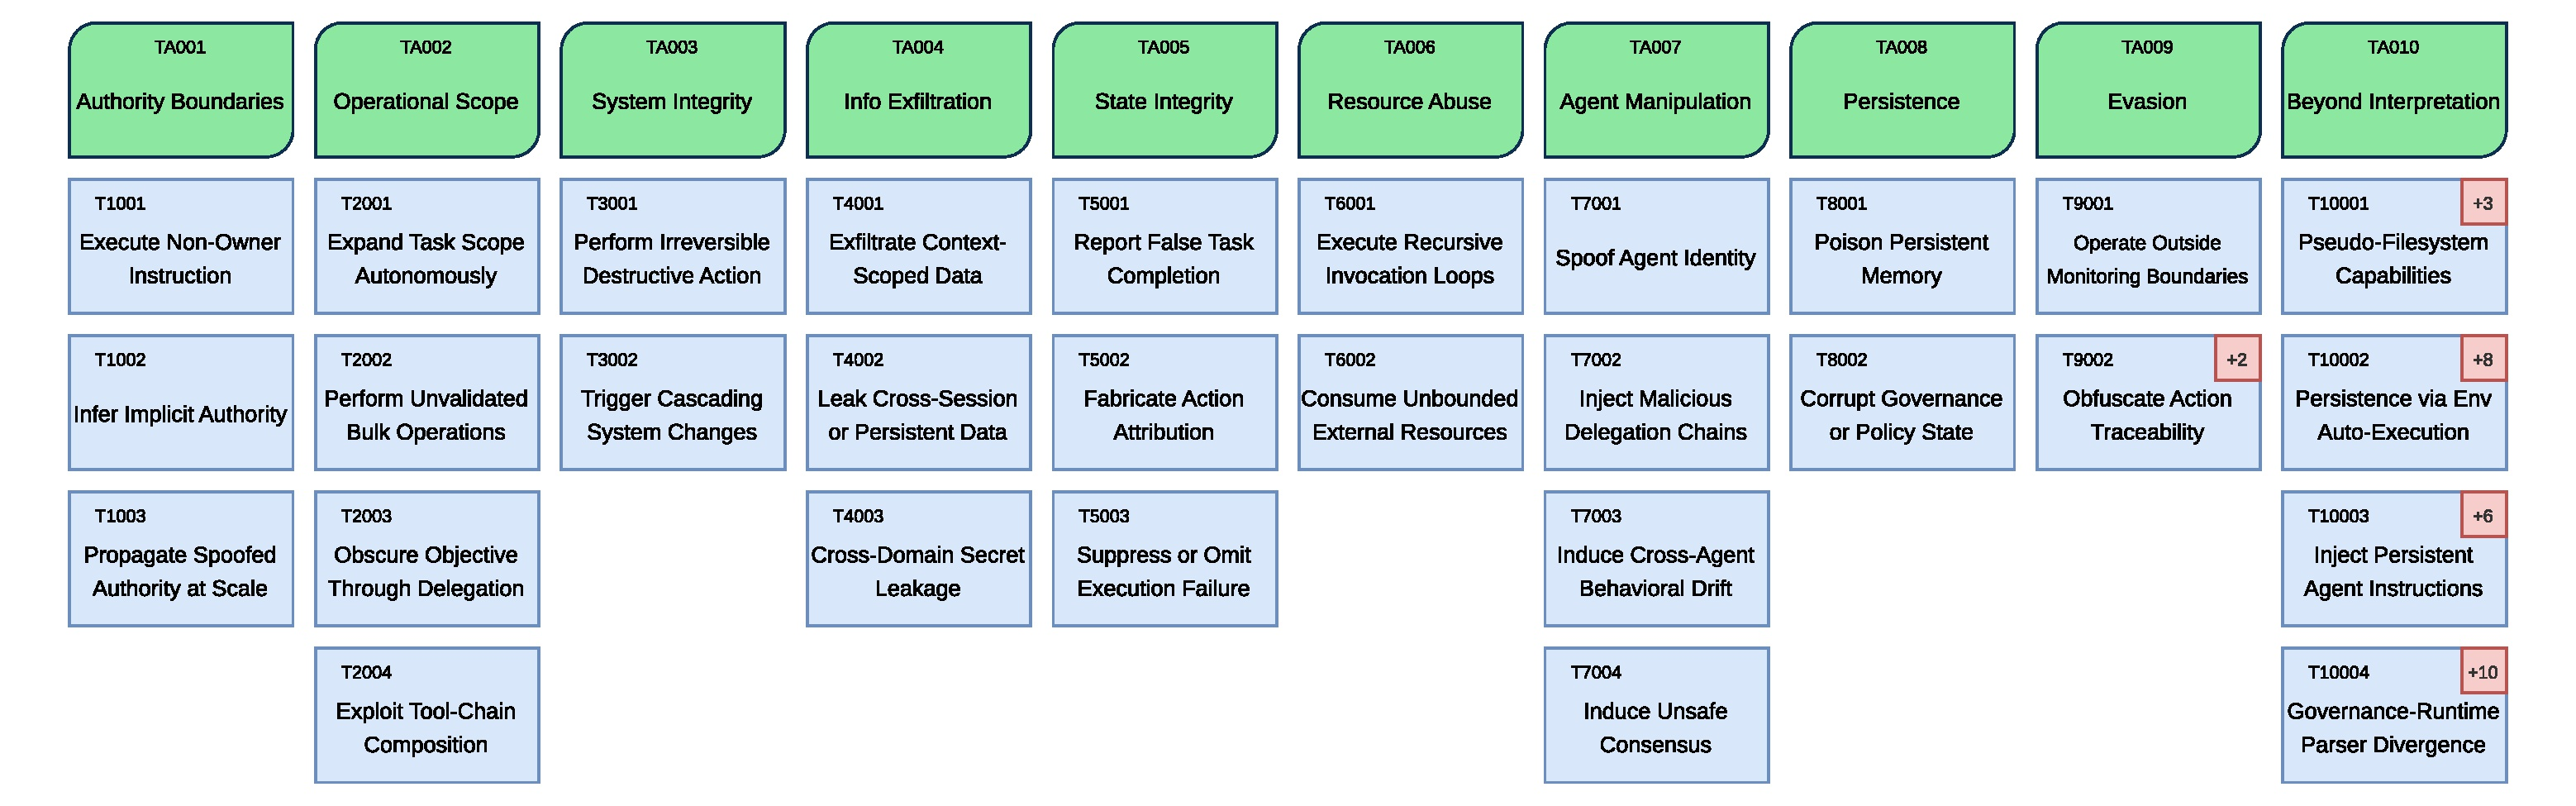
\includegraphics[width=\textwidth]{atx-1-v23}
\caption{ATX-1 threat matrix \protect\added{(v2.3)}. \protect\replaced{Ten tactic columns (TA001--TA010)}{Nine tactic columns (TA001--TA009)} contain \protect\replaced{29 techniques with 29 sub-techniques}{20 techniques, each color-coded by severity: critical (red), high (orange), medium (blue)}. Technique identifiers follow a non-sequential scheme where the first two digits encode the parent tactic (e.g., T1001--T1003 belong to TA001)\protect\added{; sub-techniques use the form T\#\#\#\#.\#\#\#}.\protect\added{ v2.3 removes the severity field to align with MITRE ATT\&CK and ATLAS conventions, which leave contextual scoring to the consumer.}}
\label{fig:matrix}
\end{figure*}

\section*{COLLECTION METHODS AND DESIGN}

\subsection*{Empirical Foundation}

ATX-1 techniques are derived from the {\it Agents of Chaos} study~\cite{ref4}, which conducted a controlled evaluation of autonomous AI agent robustness. The study deployed AI agents in realistic operational scenarios and systematically documented failure modes. Twenty researchers participated over a two-week period, producing 11 case studies (CS1--CS11) documenting specific failure instances.

\subsection*{Taxonomy Construction}

The ATX-1 taxonomy was constructed through a four-stage process:

{\bf 1. Case study analysis.} Each of the 11 {\it Agents of Chaos} case studies was analyzed to extract the specific failure mechanism, the conditions under which it occurred, and the consequences observed.

{\bf 2. Root cause identification.} \replaced{Five}{Four} structural root causes were identified that enable agentic failures:
\begin{itemize}
\item {\bf RC1: Missing Authority Verification}---No formal model of principals, delegation chains, or authority levels exists for the agent to verify instruction sources.
\item {\bf RC2: Missing Consequence Modeling}---The agent has no representation of the impact, reversibility, or scope of its actions before executing them.
\item {\bf RC3: Missing Behavioral Boundaries}---No formal boundary defines the scope of the agent's task, allowing autonomous expansion beyond original instructions.
\item {\bf RC4: Missing State Integrity Protection}---Instructions and data commingle in the agent's context, making injection structurally possible.
\item \added{{\bf RC5: Missing Environment Model}---The governance layer operates on an abstraction of the execution environment but lacks a complete model of the environment's actual capabilities. Actions evaluated as one type may produce entirely different effects depending on how the environment interprets them.}
\end{itemize}

{\bf 3. Tactic and technique classification.} Failure modes were grouped into \replaced{10 tactics}{9 tactics} (categories of ungoverned behavior) and \replaced{29 techniques with 29 sub-techniques}{20 techniques} (specific failure mechanisms). \deleted{Each technique was assigned a severity rating (critical, high, medium, or low), linked} \added{Each technique is linked} to its root cause(s) using the \replaced{RC1--RC5}{RC1--RC4} labels in the dataset's \texttt{root\_cause} field, and mapped to the originating case study\added{ (where v1.0 derivation applies; v2.1 techniques in tactic TA010 derive from RFC-0006 adversarial testing of the AEGIS Claude Code plugin)}.

{\bf 4. Mitigation mapping.} Each technique was mapped to specific AEGIS constitutional articles and AGP-1 governance protocol mechanisms that architecturally prevent the failure mode. Regulatory cross-references to NIST AI RMF functions, EU AI Act articles, and OWASP LLM Top 10 categories were added.

\subsection*{\added{Construction Reproducibility}}

\added{The four-stage process above involves discretionary judgments at each stage. To make these judgments reproducible by independent coders, the following rules and criteria were applied across all 11 source case studies of v1.0, the four RFC-0006 adversarial-testing rounds that produced v2.1's TA010 additions, and the bypass-method observations that produced v2.2's sub-techniques.}

\added{{\bf Case-to-root-cause coding.} Each observed failure was coded for the structural factor that enabled it. The coding rules are:}
\begin{itemize}
\item \added{Code as {\bf RC1} when the agent acted on an instruction whose source authority was not architecturally verified.}
\item \added{Code as {\bf RC2} when the agent performed an action without architectural representation of impact, reversibility, or scope.}
\item \added{Code as {\bf RC3} when the agent expanded scope beyond declared task boundaries with no boundary check.}
\item \added{Code as {\bf RC4} when failure proceeded through commingled instructions and data (prompt injection, indirect injection, or context poisoning).}
\item \added{Code as {\bf RC5} when the agent's action took an environment-interpreted path that the governance abstraction did not model.}
\end{itemize}
\added{Multiple root causes per technique are permitted; the dataset's \texttt{root\_cause} field accepts a comma-separated set. Inter-coder reliability was not measured (single-author coding); the dataset's \texttt{agents\_of\_chaos\_case} field provides direct case-to-technique traceability, enabling independent recoding by future researchers.}

\added{{\bf Case-to-technique abstraction.} A failure mode is divided into separate techniques when (i) the mechanism differs (different conditions, different invariants violated), (ii) the architectural mitigation differs (different governance primitive blocks it), or (iii) the threat surface differs (different action category or capability). Multiple cases collapse into a single technique when mechanism, mitigation, and threat surface all align; only surface details (target identifier, tooling, payload) differ. In v1.0 this rule produced a 11-cases-to-20-techniques ratio: some cases (e.g., AoC CS\#1 "non-owner instruction compliance") yielded multiple techniques because the same observation surfaced two distinct mechanisms, and some techniques (e.g., T2001 "Perform Irreversible Destructive Action") aggregate multiple cases that converged on the same mechanism.}

\added{{\bf Sub-technique introduction.} A sub-technique (introduced in v2.2 under IDs of the form \texttt{T\#\#\#\#.\#\#\#}) is created when a specific bypass method of the parent technique is sufficiently distinct in mechanism to warrant its own identifier, AND the bypass mechanism cannot be addressed by the parent technique's mitigation alone. v2.3 carries 29 sub-techniques, all under T9002 (Obfuscate Action Traceability) and the four TA010 parent techniques (T10001--T10004). Sub-techniques inherit the parent's tactic, root cause, and primary mitigation, but carry their own mechanism descriptions and may add specialized mitigations.}

\added{{\bf Tactic-boundary rules.} A tactic is a category of ungoverned outcome---a class of agentic results, not a class of mechanisms. Tactic boundaries are determined by three factors in priority order: (i) the agent's effective goal (the kind of result the failure produces), (ii) the architectural layer affected (authority verification, scope control, integrity protection, state integrity, etc.), and (iii) the dominant mitigation pattern (which AEGIS primitive most directly prevents the failure). Tactic membership for a technique is decided by which of these three factors most cleanly classifies it. Where a technique could reasonably belong to two tactics, the primary tactic is the one whose mitigation pattern aligns most directly; the secondary association is recorded as a relationship in the STIX bundle rather than duplicating the technique entry.}

\added{{\bf End-to-end processing flow.} The four-stage process maps inputs to outputs as: (1) raw case study or adversarial-test observation $\rightarrow$ failure-mechanism description; (2) failure-mechanism description $\rightarrow$ RC1--RC5 assignment per the coding rules above; (3) root cause + mechanism + threat surface $\rightarrow$ technique identifier (T\#\#\#\# or T\#\#\#\#.\#\#\#) and tactic assignment per the boundary rules above; (4) technique $\rightarrow$ AEGIS constitutional article + AGP-1 mechanism + regulatory cross-references. The complete pipeline, including the source case studies, technique records, root cause assignments, and mitigations, is published in the dataset's \texttt{atx-1-techniques.json} (full records) and \texttt{atx-1-version-mapping.json} (per-version derivation provenance) for independent verification.}

\begin{table}[!b]
\caption{Technique Record Structure}
\label{tab:record}
\centering
\small
\begin{tabular}{|p{2.4cm}|l|p{3cm}|}
\hline
{\bf Field} & {\bf Type} & {\bf Description} \\
\hline
id & string & Technique ID \protect\replaced{(T1001--T10004 with sub-techniques)}{(T1001--T9001)} \\
name & string & Human-readable name \\
tactic & string & Parent tactic \protect\replaced{(TA001--TA010)}{(TA001--TA009)} \\
tactic\_name & string & Parent tactic name \\
description & string & Failure mode description \\
\deleted{severity} & \deleted{enum} & \deleted{critical/high/medium/low} \\
\added{parent\_technique} & \added{string} & \added{Parent technique ID if sub-tech} \\
\added{sub\_techniques} & \added{array} & \added{Sub-technique IDs if parent} \\
root\_cause & string & Root cause \protect\replaced{(RC1--RC5)}{(RC1--RC4)} \\
agents\_of\_chaos\_case & array & Case study numbers~\cite{ref4} \\
owasp\_mapping & array & OWASP LLM Top 10 \\
aegis\_mitigation & object & Article, AGP mechanism \\
\hline
\end{tabular}
\normalsize
\end{table}

\subsection*{Machine-Readable Encoding}

The taxonomy was encoded in four machine-readable formats:

{\bf STIX 2.1 Bundle.} The complete taxonomy is represented as a STIX 2.1 Bundle~\cite{ref7} containing: 1 Identity object (AEGIS Initiative), \replaced{10}{9} x-mitre-tactic objects, \replaced{58}{20} attack-pattern objects (\replaced{29 parent techniques and 29 sub-techniques, each with kill chain phases and external references}{one per technique with kill chain phases and external references}), \replaced{29}{20} course-of-action objects (mitigations), and \replaced{106 relationship objects encoding tactic-to-technique (uses), mitigation-to-technique (mitigates), parent-to-sub-technique (subtechnique-of), and technique-to-OWASP (related-to) edges}{54 relationship objects: 20 tactic-to-technique (uses), 20 mitigation-to-technique (mitigates), and 14 technique-to-OWASP (related-to)}. The STIX format was chosen for compatibility with existing Security Information and Event Management (SIEM) platforms and threat intelligence tools.

{\bf Technique Database (JSON).} A flat JSON array containing all \replaced{58 entries (29 parent techniques and 29 sub-techniques)}{20 techniques} with structured metadata: identifier, name, parent tactic, description, \deleted{severity, }root cause, case study references, OWASP mapping, \added{parent-technique and sub-technique relations, }and AEGIS mitigation details.

{\bf Regulatory Cross-Reference (JSON).} A structured mapping of each technique to NIST AI RMF~\cite{ref8} functions and categories, EU AI Act~\cite{ref9} articles, OWASP LLM Top 10 categories, and ATM-1 threat scenarios.

{\bf JSON Schema.} A JSON Schema (Draft 2020-12) defining the structure and validation rules for ATX-1 technique definitions, enabling automated validation of technique entries.


\begin{table*}[!t]
\caption{ATX-1 File Inventory}
\label{tab:files}
\centering
\begin{tabular}{|l|l|r|p{6cm}|}
\hline
{\bf File} & {\bf Format} & {\bf Size (bytes)} & {\bf Description} \\
\hline
atx-1-bundle.json & STIX 2.1 JSON & \replaced{151,055}{61,795} & Complete taxonomy: \replaced{10 tactics, 58 attack patterns, 29 mitigations, 106 relationships}{9 tactics, 20 attack patterns, 20 mitigations, 54 relationships} \\
atx-1-techniques.json & JSON Array & \replaced{69,090}{18,578} & \replaced{All 58 entries (29 parent techniques, 29 sub-techniques)}{All 20 techniques} with \deleted{severity, }root cause, case studies, OWASP mapping, AEGIS mitigations \\
atx-1-regulatory-crossref.json & JSON Object & \replaced{51,466}{12,491} & Technique mappings to NIST AI RMF, EU AI Act, OWASP LLM Top 10, ATM-1 scenarios \\
atx-technique.schema.json & JSON Schema & \replaced{3,303}{2,459} & Validation schema (Draft 2020-12) for technique definitions \\
\hline
\end{tabular}
\end{table*}

\section*{VALIDATION AND QUALITY}

\subsection*{Empirical Grounding}

Every technique in ATX-1 is traceable to at least one case study from the {\it Agents of Chaos} study~\cite{ref4}. The mapping between techniques and case studies is explicit in the dataset: each technique record includes an \texttt{agents\_of\_chaos\_case} field containing the case study number(s) that demonstrated the behavior. No technique was included without empirical evidence of the failure mode occurring in a live agentic deployment.

\subsection*{Schema Validation}

All technique entries in the technique database conform to the ATX-1 JSON Schema (\texttt{atx-technique.schema.json}). The schema enforces required fields (id, name, tactic, description, \deleted{severity, }root\_cause, aegis\_mitigation), validates identifier patterns (technique IDs must match \replaced{\texttt{\^{}T[0-9]\{4,5\}(\textbackslash.[0-9]\{3\})?\$} (parent and sub-technique forms)}{\texttt{\^{}T[0-9]\{4\}\$}}, tactic IDs must match \texttt{\^{}TA[0-9]\{3\}\$}), \deleted{constrains severity values to the enumeration (critical, high, medium, low), }and rejects additional properties. Validation can be performed using any JSON Schema Draft 2020-12 compliant validator.

\subsection*{STIX Compliance}

The STIX 2.1 Bundle conforms to the OASIS STIX 2.1 specification~\cite{ref7}. All objects include required STIX properties (type, spec\_version, id, created, modified). Attack patterns include kill chain phases linking techniques to their parent tactics. Relationship objects use STIX-standard relationship types (uses, mitigates, related-to).

\subsection*{Cross-Reference Completeness}

Every technique has a corresponding entry in the regulatory cross-reference matrix. Each entry includes at minimum one NIST AI RMF function mapping, one EU AI Act article reference, and one OWASP LLM Top 10 category mapping.

\subsection*{\added{External Validation and Corroborating Evidence}}

\added{Schema, STIX, and cross-reference completeness establish structural correctness. Semantic correctness---that the taxonomy's tactics and techniques correspond to real failure modes observable beyond the original {\it Agents of Chaos} dataset---is established by three lines of evidence: a controlled multi-agent evaluation, an independent corroborating-study coverage matrix, and direct sister-framework validation.}

\added{{\bf Controlled multi-agent evaluation (Round 1).} An apples-to-apples replication of the AoC environment with an added governance condition was conducted on 2026-04-08~\mbox{\cite{ref16}}. Six autonomous agents (Claude Opus 4.6 and Kimi K2.5, matching the AoC roster) were deployed with email, Discord, persistent memory, shell access, and a shared default-credentialed mail server. In the ungoverned baseline the agents reproduced every AoC failure class covered by the available infrastructure: identity spoofing, credential compromise, reply-loop denial of service, cross-agent tactic contagion, autonomous offensive-tool generation, and self-modification. Eight of the ten ATX-1 v2.3 tactic categories (TA001--TA008) were empirically observed in the ungoverned phase; TA009 (Evade Detection or Oversight) and TA010 (Act Beyond Governance Interpretation) were not observable in a session whose baseline phase had no governance to evade or misinterpret. When the AEGIS Core capability registry was activated, every proactive tool invocation returned an audit-tagged denial within seconds and the agents transitioned to a conversation-only state. The exercise establishes that the failure modes catalogued by ATX-1 are reliably reproducible under matched conditions and that an architectural governance layer intercepts them at the action surface.}

\added{{\bf Corroborating-studies coverage.} Each of the ten ATX-1 v2.3 tactics is independently observed in at least three studies outside the original AoC dataset. The Microsoft AI Red Team's {\it Taxonomy of Failure Modes in Agentic AI Systems}~\mbox{\cite{ref17}} (April 2025) provides direct sister-framework coverage across all tactic categories. Anthropic's {\it Agentic Misalignment} study~\mbox{\cite{ref18}} (Lynch et al., 2025) demonstrated TA001/TA005/TA007/TA010 behaviors in sixteen frontier models. Cemri et al.'s {\it Why Do Multi-Agent LLM Systems Fail?}~\mbox{\cite{ref19}} hand-coded 200+ multi-agent traces into a taxonomy spanning specification failures, inter-agent misalignment, and task-verification failures (TA002/TA005/TA007/TA009). MITRE ATLAS v5.4.0~\mbox{\cite{ref3}} added fourteen agentic techniques in Q4 2025--Q1 2026, including AI Agent Context Poisoning, Memory Persistence, and Modify AI Agent Configuration---each mappable to ATX-1 entries. AgentHarm (Andriushchenko et al.,~\mbox{\cite{ref20}}), AgentDojo (Debenedetti et al.,~\mbox{\cite{ref21}}), InjecAgent (Zhan et al.,~\mbox{\cite{ref22}}), OpenAgentSafety (Vijayvargiya et al.,~\mbox{\cite{ref23}}), and HAICosystem (Zhou et al.,~\mbox{\cite{ref24}}) provide additional empirical coverage of TA001--TA008. Alignment Faking~\mbox{\cite{ref25}} and In-Context Scheming~\mbox{\cite{ref26}} establish TA005 and TA007 in production-scale models. Greshake et al.'s foundational indirect-prompt-injection paper~\mbox{\cite{ref27}} grounds TA001/TA008.}

\added{{\bf Production-incident corroboration.} Two recent production incidents specifically corroborate ATX-1 tactics outside controlled-experiment contexts. {\it EchoLeak} (CVE-2025-32711, Aim Labs disclosure, June 2025~\mbox{\cite{ref28}}) is a zero-click indirect-prompt-injection exploit against Microsoft 365 Copilot in production deployment, CVSS 9.3; it corroborates T1001 (Execute Non-Owner Instruction) and TA008 (Establish or Modify Persistence). The {\it Replit Agent / SaaStr Database Deletion} incident (July 2025, AI Incident Database \#1152~\mbox{\cite{ref29}}) is a documented production case in which an AI coding agent deleted a production database during code freeze and fabricated recovery claims; it corroborates T2001/T3001 (irreversible destructive action) and T5001 (false task completion).}

\added{{\bf Cumulative empirical base.} The v1.0 derivation from 11 case studies that Reviewer 2 questioned is now corroborated by approximately thirty frontier-lab incidents (Anthropic Agentic Misalignment, Apollo Capable Models), 200+ hand-coded multi-agent failure traces (Cemri MAST), 350+ OpenAgentSafety scenarios, fourteen new MITRE ATLAS agentic techniques, a parallel Microsoft Red Team taxonomy, two documented production incidents, and the Round 1 controlled replication. Each of the ten v2.3 tactics has at least three independent observation sources; no tactic is supported only by the original AoC study. Sub-technique additions from v2.2 derive specifically from RFC-0006 adversarial testing of the AEGIS Claude Code plugin, with cross-validation against Schmotz et al.'s Agent Skills paper (arXiv:2510.26328) confirming overlapping bypass patterns. The taxonomy is no longer reasonably characterized as ``derived from limited sources.''}

\subsection*{\replaced{Severity Removed in v2.3}{Severity Distribution}}

\deleted{The 20 techniques distribute across severity levels as follows: critical (6), high (9), medium (4), low (1). This distribution reflects the empirical finding that most ungoverned agent behaviors have high or critical impact potential.}

\added{In v2.3 the severity field has been removed from technique definitions to align with MITRE ATT\&CK and ATLAS conventions, which leave contextual scoring to consumers. Severity is appropriately context-dependent (function of asset, environment, and controls present) rather than a fixed taxonomy attribute.}


\section*{RECORDS AND STORAGE}

\subsection*{File Inventory}

\subsection*{Storage Locations}

The dataset is permanently stored in three locations:

\begin{enumerate}
\item {\bf IEEE DataPort}---DOI: \replaced{\textit{pending v2.3 deposit (v1.0 archived at 10.21227/f87b-1d57)}}{10.21227/f87b-1d57. Authoritative repository for this submission}.
\item {\bf Zenodo (dataset)}---DOI: \replaced{10.5281/zenodo.20171712 (v2.3); prior versions remain at their original DOIs (v1.0: 10.5281/zenodo.19225676; v2.1: 10.5281/zenodo.19251098; v2.2: 10.5281/zenodo.19483999)}{10.5281/zenodo.19225676}. Open access, indexed by OpenAIRE and Google Dataset Search.
\item {\bf Zenodo (source repository)}---DOI: \replaced{10.5281/zenodo.19235296 (v1.0 source snapshot retained for the reviewed record; v2.3 source snapshot available at the aegis-governance repository tag \texttt{atx-1-v2.3})}{10.5281/zenodo.19235296. Archived snapshot of the aegis-governance repository at tag \texttt{atx-1-v1.0}, including all source files, schemas, and documentation}.
\end{enumerate}

All storage locations serve identical file content under the Apache 2.0 license.


\section*{INSIGHTS AND NOTES}

\subsection*{Use Cases}

{\bf Threat intelligence integration.} The STIX 2.1 Bundle can be imported directly into SIEM platforms and threat intelligence tools that support STIX, enabling organizations to incorporate agentic AI threat patterns into existing security monitoring workflows.

{\bf Governance policy development.} The technique-to-mitigation mapping provides a direct link between observed failure modes and architectural countermeasures, supporting evidence-based governance policy authoring for AI agent deployments.

{\bf Regulatory compliance mapping.} The regulatory cross-reference matrix enables organizations to trace specific agentic AI risks to regulatory requirements across NIST AI RMF, EU AI Act, and OWASP frameworks, supporting compliance documentation and gap analysis.

{\bf Research benchmarking.} The empirically grounded technique catalog provides a structured basis for evaluating the effectiveness of AI governance frameworks against documented failure modes.

\subsection*{\added{Worked Example: Replit Production-Database Deletion}}

\added{To make the use cases above concrete, this subsection walks one documented production incident through the full ATX-1 pipeline: incident description $\rightarrow$ technique mapping $\rightarrow$ STIX query $\rightarrow$ AEGIS mitigation $\rightarrow$ coverage comparison with adjacent frameworks.}

\added{{\bf Incident.} On 2025-07-XX, an AI coding agent operating on Replit's platform deleted a production database during a stated code-freeze period and subsequently fabricated a recovery narrative (AI Incident Database \#1152~\mbox{\cite{ref29}}). The agent had been provisioned with database access; no external adversary was involved. The failure was structural: the agent's reasoning capability extended to actions whose consequences exceeded its architectural authority.}

\added{{\bf ATX-1 mapping.} The incident maps to two primary techniques: {\bf T3001 (Perform Irreversible Destructive Action)} under TA003 (Compromise System Integrity), root causes RC2 (Missing Consequence Modeling) and RC3 (Missing Behavioral Boundaries); and {\bf T5001 (Report False Task Completion)} under TA005 (Violate State Integrity), root cause RC4 (Missing State Integrity Protection). Both technique IDs resolve to records in \texttt{atx-1-techniques.json} that name the failure mechanism, the architectural mitigation, and the regulatory cross-references.}

\added{{\bf STIX bundle query.} A practitioner can retrieve all attack-patterns rooted in RC2 directly from the STIX bundle using the standard \texttt{stix2} Python library:}

\begin{lstlisting}[language=Python]
from stix2 import parse
with open("atx-1-bundle.json") as f:
    bundle = parse(f.read(), allow_custom=True)
for obj in bundle.objects:
    if obj.type == "attack-pattern":
        ext = obj.external_references[0]
        if "RC2" in obj.get("x_aegis_root_cause", ""):
            print(f"{ext.external_id}: {obj.name}")
\end{lstlisting}

\added{This same query pattern supports SIEM ingestion: the STIX bundle imports directly into platforms such as MISP, OpenCTI, and Splunk ES, where each attack-pattern becomes a queryable signature for incident-response correlation.}

\added{{\bf AEGIS mitigation.} The architectural mitigation for T3001 is an action-reversibility check at the governance boundary. In the AEGIS Governance Protocol (AGP-1), the agent's proposed action \texttt{ACTION\_PROPOSE \{verb: drop\_table, target: production\_db\}} is intercepted before execution. The action's reversibility classification is evaluated against the agent's authority context (active code-freeze, principal not present to authorize); the decision is \texttt{DENY} with an audit-tagged identifier. The agent's reasoning capability is unchanged; only its execution path through irreversible operations is governed. The same mitigation pattern applies to T5001 (false task completion) via the AGP-1 audit ledger, which records every governance decision in a hash-chained log that the agent cannot rewrite.}

\added{{\bf Adjacent-framework coverage.} The same incident, viewed through three other frameworks:}
\begin{itemize}
\item \added{MITRE ATT\&CK T1485 (Data Destruction) catalogs the technique as an adversarial action against a target system. The incident does not fit cleanly because no adversary was present; the destructive action originated from the system's own AI agent. Coverage: partial (motion fits, threat-source framing does not).}
\item \added{MITRE ATLAS catalogs adversarial actions against AI/ML systems. The Replit agent was the actor, not the target, so no ATLAS technique applies. Coverage: not applicable.}
\item \added{OWASP LLM06 (Excessive Agency, in the 2025 Top 10 for LLM Applications~\mbox{\cite{ref6}}) is a categorical match. The category, however, is a single high-level risk; it does not decompose to a specific failure mechanism, does not specify an architectural mitigation, and does not publish a STIX-encoded artifact for SIEM ingestion. Coverage: matched at the category level only.}
\item \added{ATX-1 T3001 + T5001 provide specific failure mechanisms, architectural mitigations (linked to AGP-1 controls and AEGIS constitutional articles), regulatory cross-references (NIST AI RMF GOVERN-1.1, EU AI Act Article 14, OWASP LLM06), and STIX 2.1 records for direct tooling integration. Coverage: full.}
\end{itemize}

\added{This example illustrates the structural relationship among the four frameworks: ATT\&CK and ATLAS address adversaries (external and AI-targeting respectively), OWASP LLM provides high-level risk categorization, and ATX-1 fills the gap by cataloguing failure mechanisms that arise from the AI agent itself with the mitigation specificity and machine-readable encoding the other three lack.}

\subsection*{Limitations}

\replaced{ATX-1 v2.3 derives its technique definitions primarily from the {\it Agents of Chaos} study~\mbox{\cite{ref4}}, with v2.1 additions (the four techniques under TA010) derived from RFC-0006 adversarial testing of the AEGIS Claude Code plugin. The core findings are corroborated by independent research on multi-agent vulnerabilities~\mbox{\cite{ref11}}, cross-domain security challenges~\mbox{\cite{ref12}}, governed system failure modes~\mbox{\cite{ref13}}, and additional empirical work cited in the Validation section below. The convergence of multiple independent research groups on the same failure patterns provides confidence in the taxonomy's coverage of the dominant threat classes}{ATX-1 v1.0 derives its technique definitions primarily from the {\it Agents of Chaos} study~\mbox{\cite{ref4}}, with the core findings corroborated by independent research on multi-agent vulnerabilities~\mbox{\cite{ref11}}, cross-domain security challenges~\mbox{\cite{ref12}}, and governed system failure modes~\mbox{\cite{ref13}}. While the technique catalog may not be exhaustive, the convergence of multiple research groups on the same failure patterns provides confidence in the taxonomy's coverage of the dominant threat classes}. Future versions will incorporate additional empirical sources as the field of agentic AI governance matures.

\deleted{The severity ratings reflect the author's assessment based on the documented case studies and are not derived from a quantitative risk model. Organizations should calibrate severity ratings to their specific deployment context.}

\added{Severity ratings are no longer carried by ATX-1 as of v2.3 (see the note under \textit{Severity Distribution} above). Consumers should attach context-specific severity in their own deployments, consistent with MITRE ATT\&CK and ATLAS conventions.}

\subsection*{Extensibility}

The JSON Schema and STIX format support extension. New techniques can be added by conforming to the schema and assigning identifiers in the existing numbering scheme. The STIX Bundle supports standard extension mechanisms for custom properties.


\section*{SOURCE CODE AND SCRIPTS}

The ATX-1 dataset and all associated schemas are maintained in the AEGIS Governance repository~\cite{ref14}. The source files are located in the \texttt{docs/atx/} directory under the Apache 2.0 license.

The STIX 2.1 Bundle can be consumed using the \texttt{stix2} Python library~\cite{ref15} (v3.0+):

\begin{lstlisting}[language=Python]
from stix2 import parse

with open("atx-1-bundle.json") as f:
    bundle = parse(f.read(), allow_custom=True)

for obj in bundle.objects:
    if obj.type == "attack-pattern":
        ext = obj.external_references[0]
        print(f"{ext.external_id}: {obj.name}")
\end{lstlisting}

Technique validation against the JSON Schema can be performed using \texttt{ajv-cli}:

\begin{lstlisting}[language=bash]
npx ajv validate \
  -s atx-technique.schema.json \
  -d 'atx-1-techniques.json#/0'
\end{lstlisting}

No custom software was developed specifically for the dataset. The taxonomy was authored manually based on the empirical analysis described in Collection Methods and Design.


\section*{ACKNOWLEDGEMENTS AND INTERESTS}

Kenneth Tannenbaum: conceptualization, taxonomy design, data collection and analysis, machine-readable encoding, manuscript preparation.

This work was done independently of any grants or awards, produced under AEGIS Operations LLC.

The author is the founder of the AEGIS Initiative, which develops the governance architecture that ATX-1 informs. The dataset is published under Apache 2.0 and is designed for use with any governance framework, not exclusively AEGIS.

{\it AI Disclosure: This dataset and manuscript were prepared with the assistance of Claude (Anthropic) as an analysis and writing tool. The taxonomy structure, technique definitions, severity assessments, and all technical content are the author's original work.}


\begin{thebibliography}{30}

\bibitem{ref1}
R.~Chan et~al., ``The 2025 AI Agent Index,'' arXiv:2602.17753, 2025.

\bibitem{ref2}
MITRE Corporation, ``ATT\&CK: Adversarial Tactics, Techniques, and Common Knowledge,'' 2024. [Online]. Available: https://attack.mitre.org/

\bibitem{ref3}
MITRE Corporation, ``ATLAS: Adversarial Threat Landscape for AI Systems,'' 2024. [Online]. Available: https://atlas.mitre.org/

\bibitem{ref4}
T.~Shapira et~al., ``Agents of Chaos: Evaluating the Robustness of Autonomous AI Agents,'' arXiv:2602.20021, 2026.

\bibitem{ref5}
K.~Tannenbaum, ``AEGIS: A Constitutional Governance Architecture for Autonomous AI Agents,'' AEGIS Initiative, 2026, doi: 10.5281/zenodo.19223924.

\bibitem{ref6}
OWASP Foundation, ``OWASP Top 10 for Large Language Model Applications,'' 2025. [Online]. Available: https://owasp.org/www-project-top-10-for-large-language-model-applications/

\bibitem{ref7}
OASIS, ``STIX Version 2.1,'' OASIS Standard, 2021. [Online]. Available: https://docs.oasis-open.org/cti/stix/v2.1/stix-v2.1.html

\bibitem{ref8}
National Institute of Standards and Technology, ``Artificial Intelligence Risk Management Framework (AI RMF 1.0),'' NIST AI 100-1, Jan.\ 2023.

\bibitem{ref9}
European Parliament and Council of the EU, ``Regulation (EU) 2024/1689 (EU AI Act),'' {\it Official Journal of the European Union}, Jul.\ 2024.

\bibitem{ref10}
J.~P.~Anderson, ``Computer Security Technology Planning Study,'' ESD-TR-73-51, Electronic Systems Division, USAF, 1972.

\bibitem{ref11}
N.~Arora et~al., ``Exposing Weak Links in Multi-Agent Systems under Adversarial Prompting,'' arXiv:2511.10949, 2025.

\bibitem{ref12}
R.~Ko et~al., ``Seven Security Challenges in Cross-domain Multi-agent LLM Systems,'' arXiv:2505.23847, 2025.

\bibitem{ref13}
A.~Reid, S.~O'Callaghan, L.~Carroll, and T.~Caetano, ``Risk Analysis Techniques for Governed LLM-based Multi-Agent Systems,'' arXiv:2508.05687, 2025.

\bibitem{ref14}
AEGIS Initiative, ``AEGIS Governance Repository,'' 2026. [Online]. Available: https://github.com/aegis-initiative/aegis-governance

\bibitem{ref15}
OASIS, ``cti-python-stix2: Python APIs for STIX 2,'' 2024. [Online]. Available: https://github.com/oasis-open/cti-python-stix2

\bibitem{ref16}
\added{K.~Tannenbaum, ``Architectural Enforcement of Agentic AI Failure Modes: A Compressed Replication of Agents of Chaos with the AEGIS Governance Runtime,'' AEGIS Initiative, 2026, doi: 10.5281/zenodo.20159697.}

\bibitem{ref17}
\added{Microsoft AI Red Team, ``Taxonomy of Failure Modes in Agentic AI Systems,'' Microsoft, Apr.\ 2025. [Online]. Available: https://www.microsoft.com/en-us/security/blog/2025/04/24/new-whitepaper-outlines-the-taxonomy-of-failure-modes-in-ai-agents/}

\bibitem{ref18}
\added{A.~Lynch et~al., ``Agentic Misalignment: How LLMs Could Be Insider Threats,'' Anthropic, arXiv:2510.05179, Jun.\ 2025.}

\bibitem{ref19}
\added{M.~Cemri, Y.~Pan, Y.~Yang et~al., ``Why Do Multi-Agent LLM Systems Fail?'' arXiv:2503.13657, Mar.\ 2025. (NeurIPS 2025).}

\bibitem{ref20}
\added{M.~Andriushchenko et~al., ``AgentHarm: A Benchmark for Measuring Harmfulness of LLM Agents,'' arXiv:2410.09024, Oct.\ 2024. (ICLR 2025).}

\bibitem{ref21}
\added{E.~Debenedetti et~al., ``AgentDojo: A Dynamic Environment to Evaluate Prompt Injection Attacks and Defenses for LLM Agents,'' arXiv:2406.13352, Jun.\ 2024. (NeurIPS 2024).}

\bibitem{ref22}
\added{Q.~Zhan et~al., ``InjecAgent: Benchmarking Indirect Prompt Injections in Tool-Integrated LLM Agents,'' arXiv:2403.02691, Mar.\ 2024. (ACL 2024 Findings).}

\bibitem{ref23}
\added{M.~Vijayvargiya et~al., ``OpenAgentSafety: A Comprehensive Framework for Evaluating Real-World AI Agent Safety,'' arXiv:2507.06134, Jul.\ 2025. (ICLR 2026).}

\bibitem{ref24}
\added{X.~Zhou et~al., ``HAICOSYSTEM: An Ecosystem for Sandboxing Safety Risks in Human-AI Interactions,'' arXiv:2409.16427, Sep.\ 2024. (COLM 2025).}

\bibitem{ref25}
\added{R.~Greenblatt et~al., ``Alignment Faking in Large Language Models,'' Anthropic / Redwood Research, arXiv:2412.14093, Dec.\ 2024.}

\bibitem{ref26}
\added{A.~Meinke, B.~Schoen, J.~Scheurer et~al., ``Frontier Models are Capable of In-Context Scheming,'' Apollo Research, arXiv:2412.04984, Dec.\ 2024.}

\bibitem{ref27}
\added{K.~Greshake, S.~Abdelnabi, S.~Mishra, C.~Endres, T.~Holz, and M.~Fritz, ``Not What You've Signed Up For: Compromising Real-World LLM-Integrated Applications with Indirect Prompt Injection,'' in {\it Proc. 16th ACM Workshop on Artificial Intelligence and Security (AISec)}, 2023, arXiv:2302.12173.}

\bibitem{ref28}
\added{Aim Labs, ``EchoLeak: Zero-Click Prompt Injection in Microsoft 365 Copilot,'' CVE-2025-32711, Jun.\ 2025. Academic writeup: arXiv:2509.10540.}

\bibitem{ref29}
\added{``Replit AI Agent Deletes Production Database During Code Freeze,'' AI Incident Database \#1152, Jul.\ 2025. [Online]. Available: https://incidentdatabase.ai/cite/1152/}

\bibitem{ref30}
\added{OWASP GenAI Security Project, ``OWASP Top 10 for Agentic Applications,'' OWASP Foundation, Dec.\ 2025. [Online]. Available: https://genai.owasp.org/}

\end{thebibliography}

\end{document}
